\chapter[Large Datasets and CNN]{Large Datasets and Big Models}

\section{Why deep networks?}
Several studies have demonstrated that for certain task the performance of certain machine learning models are better with the increasing complexity of the model working on the same set of data. That is when you have a huge amount of data more complex models have better performances. 
The graph showed below explains such a feature:
\begin{figure}[h]
    \centering
    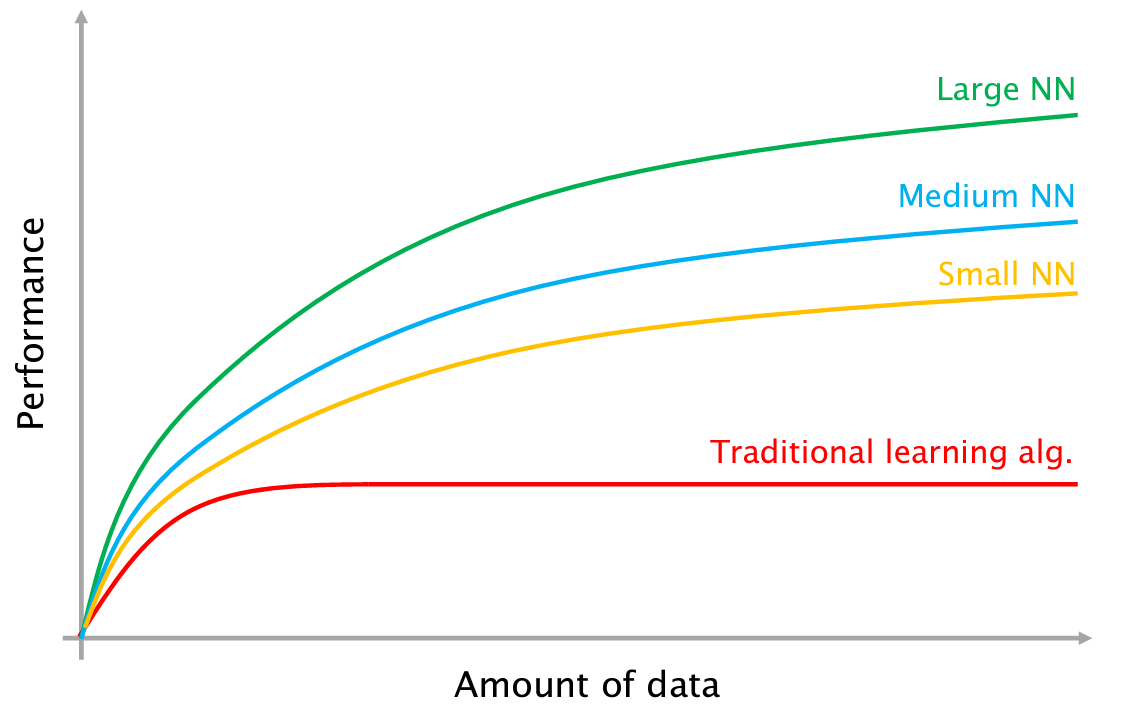
\includegraphics[scale=0.4]{img/perf.png}
    \caption{Amount of data vs Performances varying the model}
\end{figure}
The classical example can be done is the following: imagine that a classification task on images have to be performed, especially whether the figures are colored, there is an exploding number of features. A classical fully connected neural network has very bad performance with respect to a deep network, for example a \textit{Convolutional Neural Network}.

\section{Aspects related to large datasets and deep networks}
We have seen in the past chapter, when a neural network has to be trained there is always a thread-off between bias and variance to manage. There are several aspects related to deep models which ought to be taken into account. In the following the most important aspects are presented.

\subsection{Regularizing neural networks}
How we mentioned in the past paragraphs, the \textit{regularization} is a technique which is used to face the problem of overfitted models. Such a technique consists of introducing into the \textit{cost function} $J(w,b)$ a term which depends on the parameters.
For a single neuron the loss function is modified as follows:
\begin{equation} \label{eq:l2reg}
    J(w,b)=\frac{1}{m} \sum_{i=1}^{m} {\text{Loss}(\hat{y}^{(i)}, y^{(i)})+
    {\color{red}\frac{\lambda}{2m}{\Vert w \Vert_2^2}}}
\end{equation}
The term in red is the \textbf{regularization term}, its effect is to keep the complete set of features without eliminate nothing, the difference is that for certain parameters (associated to certain features) the magnitude is very small or equal to zero in order to reduce in some way the complexity of the model which was causing the overfitting phenomenon. The one showed in the (\ref{eq:l2reg}) is the $\ell_2$-norm regularization, since the $\ell_2$-norm of the vector $w$ of the weights multiplied by a parameter $\lambda$ (regularization parameter) is added to the original functional. Other types of regualarizations can be used for example the $\ell_1$-norm. The regularization term, then has the hyperparameter $\lambda$ which is crucial. In particular:
\begin{itemize}
    \itemsep-0.3em
    \item $\lambda$ \textit{very small} is associated with an \textbf{almost full model}; 
    \item $\lambda$  \textit{very high} is associated with a model whose parameters are very small, and so to a very simplified model.
\end{itemize}
For a neural network of $L$ layers the $J$ functional becomes:
\begin{equation}
    L(W^{[1]}, b^{[1]}, W^{[1]}, b^{[2]}, ...)=\frac{1}{m} \sum_{i=1}^{m} {\text{Loss}(\hat{y}^{(i)}, y^{(i)})}+
    {\color{red}\sum_{l=1}^{L}{\Vert{W^{[l]}}\Vert_F^2}}
\end{equation} 
Where {$\Vert{W}\Vert_F^2$} is the \textit{Frobenius Norm} which is the generalization of the $\ell_2$-norm in the case of matrices. Intuitively the goal is obtaining $\Vert{W}\Vert_F^2$ close to zero, since near the origin the $g(z)$ behaves in a linear way, this avoids the data to be overfitted.\\
Clearly, since $J$ is modified, also the gradient descent is modified. More specifically a term 
\begin{equation*}
    \frac{\lambda}{m} W^{[l]}
\end{equation*}
is added. This results in the update step, in multiplying the weights by a quantity equal to 
\begin{equation*}
    1-\alpha\frac{\lambda}{m}
\end{equation*}
the the higher $\lambda$ the lower such a contribution which shrinks the parameters more and more near to the origin. This is the reason why the $\ell_2$-norm regularization is also called \textit{weight decay}.

\subsection{Dropout}
\textbf{Dropout} is another regularization technique in which for each layer of the network a certain threshold is fixed and this is associated to the probability of keeping or removing one or more of its neurons. The reason why such an apparently strange technique works very well is that removing some units from each layer according to the fixed probability the structure of the network is simpler resulting in a reducing in the overfitting entity. The dropout has to be disabled in the test phase, because is something of helpful only in the phase of construction of the model.

\subsection{Data augmentation}
Among the techniques to reduce overfitting \textbf{data augmentation} is used when the dataset is not so rich. This helps us in obtaining new data starting from the ones in the original dataset. Some distortion are introduced in a way that the model perceives that information as different ones. In the field of image classification this is a very used technique. More specifically when Convolutional Neural Networks grew larger in the 90s, there was a lack of data to use, especially considering that a portion of the dataset was devoted to the testing phase. It was proposed to \textit{perturb existing data} with \textit{affine transformation}, in order to create new examples with the same labels. The most common transformation are: geometric, color space transformation and a sort of noise injection. In the following two examples  are showed with a cat image and with a number.

\begin{figure}[h]
    \centering
    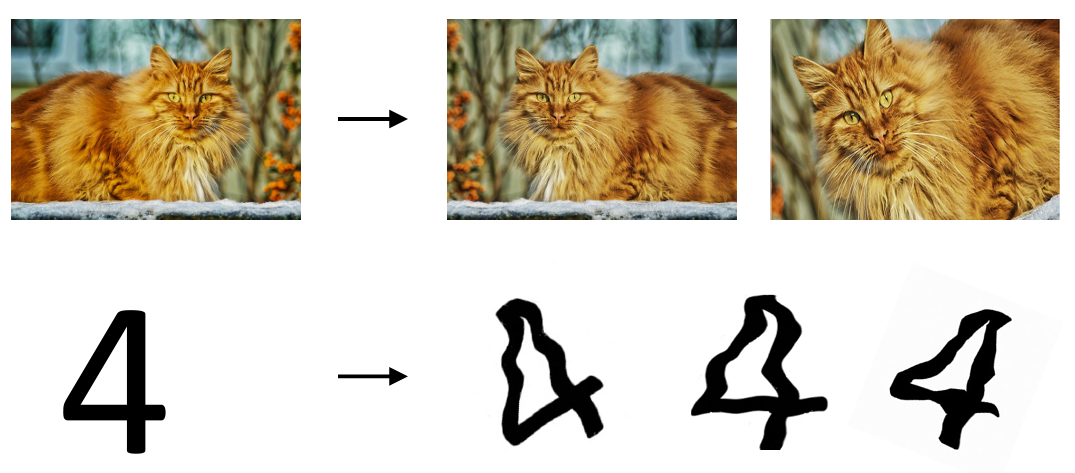
\includegraphics[scale=0.5]{img/data_sug.png}
    \caption{Data augmentation }
\end{figure}

\subsection{Mini-batch gradient descent}
Especially for bigger models than a classical multi-layer perceptron using the "classical" gradient descent could be very slow, since for each one the iterations, which hopefully, bring to the convergence, the \textbf{entire dataset} is scanned. This would have made the procedure very slow! That we called "classical Gradient Descent" is also known as \textbf{Batch Gradient Descent}.\\
The alternative here is to split the entire batch of data constituting the dataset into \textbf{mini-batch}. Doing in this way, one step of Gradient Descent passes through a subset of the data making the computations faster. When all of the batches of the training set have been used an \textbf{epoch} has been completed. In the classical approach one epoch is associated to one step of gradient descent, on the other hand if we split the dataset into $M$ batches, $M$ gradient steps are done in one epoch.

\subsubsection{Loss function and mini-batch gradient descent}
It is not supposed to be a surprise if we state that the shape of cost function through the different iterations is not so smooth as in the \textit{batch version}, since at each step different data are used.

\begin{figure}[h]
    \centering
    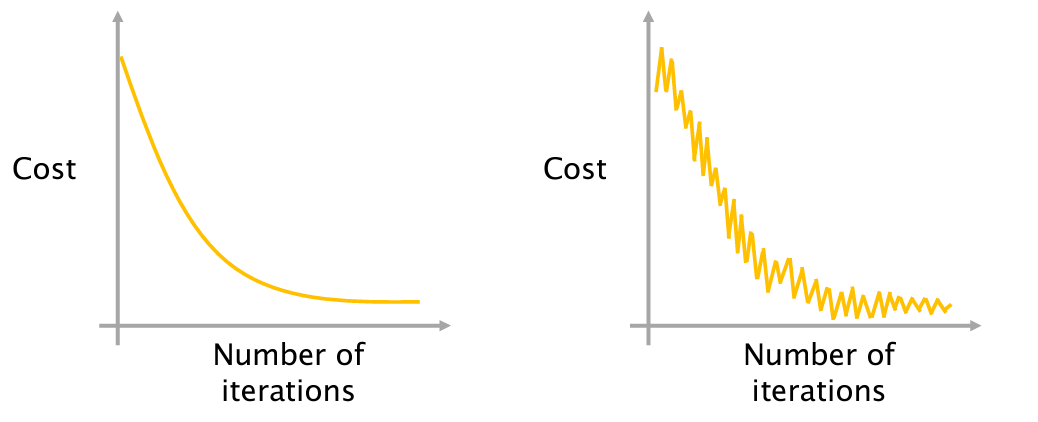
\includegraphics[scale=0.4]{img/mini-batch-iterations.png}
    \caption{\# of iterations vs Cost (Batch vs Mini-Batch)}
\end{figure}

\subsubsection{Mini-batch size}
In the case the size of a mini-batch is 1, we talk about the \textbf{stochastic gradient descent} ot the opposite if the batch size coincides with the cardinality of the dataset, then batch GD = mini-batch GD. If we go deeper into this aspect by analysing the level curves that from the initial conditions bring us to the minimum, the case of batch gradient descent is the ideal one since the path from the initial value to the minimum is straight. The same does not occur in the case SGD is used. In the practical case a value for the mini-batch size between 1 and $m$ must be chosen, this choice results in another \textit{hyperparameter}.

\begin{figure}[h]
    \centering
    \subfigure[size=m]{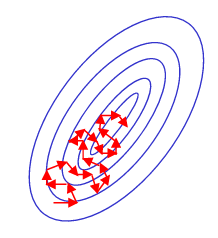
\includegraphics{img/minibatch_contourplot.png}} \quad 
    \subfigure[size=1]{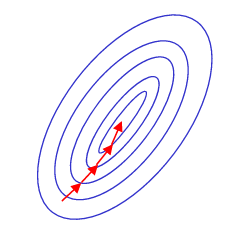
\includegraphics{img/batch_contourplots.png}}
    \caption{Contour plots varying batch size}
\end{figure}

The suggestion in this field is to use the original version of gradient descent with a small dataset (eg. 2000 examples), otherwise typical sizes for mini-batches are 64, 128, 256 and so on. In order to avoid problems, you are supposed to be sure that it fits in the used CPU/GPU.

\subsection{The problem of local minima}
Let us make another objection on the cost function, we have seen which is a fundamental building block of our machine learning task. Now, after having combined the several layers of the network (each one of the layers use different activation functions) is the $J(w,b)$ convex? The answer is NO. The functional we obtain loses its convexity with the increasing complexity of the network. However, thanks to the structure of the final cost function, the probability to be trapped into a local optima is very low. \texttt{part to be rewiewed}

\begin{figure}[h]
    \centering
    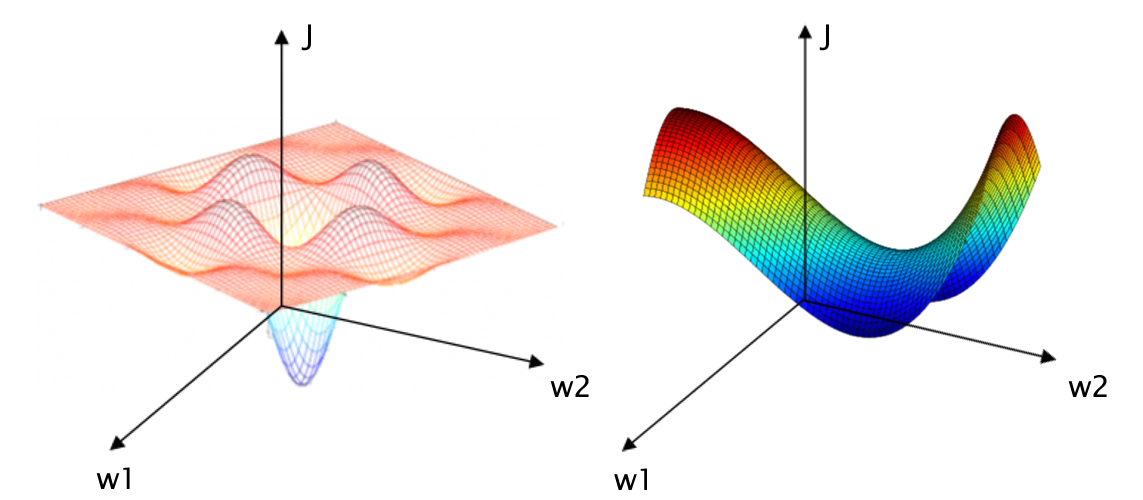
\includegraphics[scale=0.6]{img/Jnocvx.png}
    \caption{Cost function for a NN with two parameters}
\end{figure}
In the case that in the functional there are \textbf{plateaus} can be a problem, since being the derivatives constant the learning is very slow.

\subsection{Exploding/Vanishing gradients and initialization in DNN}
The \textbf{exploding} and \textbf{vanishing gradient} are both problems related to very deep networks were the weights are too high or too low, in the former case the computed gradients \textit{grow exponentially}, in the latter case they decrease their own value till they become null.\\
For sake of simplicity suppose that the activation function is a line $g(z)=z$, moreover let $b=0$, than the predicted output $\hat{y}$ has the shape:

\begin{equation*}
    \hat{y}=W^{[L]}W^{[L-1]}...W^{[1]}{x}
\end{equation*}
Whether for example the weights were all equal to 1.5 the $\hat{y}$ would be very big, on the other hand, whether all of the weights were 0.5 there would be an \textit{exponential decreasing} of the activations, a similar situation occur for the derivatives. In deep neural networks not rarely such problems appear, and differently from the \textbf{shallow neural networks} a more accurate technique aimed to cope with them is needed. In particular, has been empirically demonstrated that such a problem is reduced when the weights $w^{[l]}$ of a certain layer $l$ are randomly initialized with a value in the range $[0,1]$ multiplied by the standard deviation
\begin{equation*}
    \sigma^{[l]}=\sqrt{\frac{1}{n^{[l-1]}}}
\end{equation*}
where $n^{[l-1]}$ is the number of unit of the $(l-1)$-th layer (previous layer).


\subsection{Batch normalization}
We have seen in the introduction in order to speedup the training phase a proper choice when data are on completely different scales is the \textbf{normalization}. To better clarify such an aspect, we can say that 2 different steps are performed\footnote{
    The same $\mu$, $\sigma$ are supposed to be used in order to normalize also the remaing parts of the dataset: \textit{test} and \textit{development} set.
}:
\begin{itemize}
    \itemsep-0.3em
    \item Subtract the mean $\mu$ computed on that feature on the whole dataset (to be computed a-priori); 
    \item Divide by standard deviation $\sigma$ computed always over the whole training set for that specific feature.
\end{itemize}
In the past years, scientists working on deep learning has showed that if such a normalization is applied also for the activations (more specifically to the linear part $z$), then the learning of the parameters for a certain level is \textbf{faster}. This is the main feature behind the \textbf{batch normalization}. We know that for a certain layer $l$, we can compute the activation $A^{[l]}$ as:
\begin{equation*}
    A^{[l]}=g(Z^{[l]})
\end{equation*}
then the \textit{batch normalization} procedure is carried out as follows:
\begin{itemize}
    \itemsep-0.3em
    \item For each layer $l$, for each feature $i$, the mean $\mu$ and variance $\sigma^2$ are computed.
    \item The normalized data $Z^{[l](i)}_{\text{norm}}$ are obtained as follows:
    \begin{equation*}
        Z^{[l](i)}_{\text{norm}}=\frac{
            Z^{[l](i)}-\mu
        }{
            \sqrt{\sigma^2+\varepsilon}
        }
    \end{equation*}
    \item For the training phase the following data are used:
    {\large{
        \begin{equation}\label{eq:batch_normalization}
            \tilde{Z}^{[l](i)}={\color{red}\gamma}{Z}^{[l](i)}_{\text{norm}}+{\color{red}\eta}
        \end{equation}
    }}
\end{itemize}
This approach, fortunately or not, leads with it other hyperparameters which are $\varepsilon, \gamma, \eta$. Moreover, just to further complicate the situation, for each layer different $\gamma^{[l]}$ and $\eta^{[l]}$ could be used. It is interesting now, after this formal description to better understand what are the guidelines leading to batch normalization and what is its effect. \\
In principle when I perform the normalization on the input data (remind they are also called 0-layer activations) after the first forward step, I completely lose the effect since the first-layer activations are something very different than the \textit{normal} range. Moreover batch normalization also has a \textit{slight regularization effect}: the fact that mean and variance are computed with respect to that mini-batch adds similarly than \textit{dropout} adds some noise to each hidden layer activations. 

\subsection{Softmax Layer}
At the beginning we have seen that the hypotesis (later called \textit{activation}) can be interpreted as the probability of belonging to a certain class given the records X, but how can be interpreted as a result? We would like to have on the last layer $L$ a some probability that, differently from the other sum up to one. For this reason, very often in the neurons of the last layer a particular activation function is used: 
\begin{equation} \label{eq: Softmax}
    a_i^{[L]}=\frac{t_i}{\sum_{j=1}^{n^{[L]}}{t_j}}
\end{equation}
where $a_i^{[L]}$ is the activations for the $i-th$ unit in layer $L$, and $t_i\doteq{e^{z_{i}^{[L]}}}$. When the softmax activation function is used, the loss function to be used is the following (\textit{for a single training sample}): 
\begin{equation}\label{eq:loss_softmax}
    \text{Loss}^{(i)}(\hat{y}, y)=\sum_{j=1}^{n^{[L]}} -y_{j} \log(\hat{y}_j)
\end{equation}
Note that $n^{[L]}$ is the number of classes, in this case for the $m$ training samples the \textbf{one-hot encoding} is used for representing the labels, in particular:
\begin{equation}\label{eq: one_hot}
    Y=\big[
        y^{(1)} \quad y^{(2)} \quad ... \quad y^{(m)}
    \big] = \begin{bmatrix}
        0&1& &0\\
        1&0& &1\\
        0&0&...&0\\
        0&0& &0
    \end{bmatrix} \in \mathbb{R}^{n^{[L]}, m}
\end{equation}
For each example a vector in which only $i$-th element is one with correspondence to the true class for that record.

\subsection{Transfer learning}
Especially in the field of deep learning, rarely one starts from scratches to develop the neural network. There are several motivations for which this is not happening, a common one is that there is lack of resources. To the aim to train certain models several dozens of GPU could be required... The \textbf{Transfer learning} aids us to cope with this problem. It consists in the use of a part of a pre-trained model in order to use its parameters as input features for a task of us. Then, by doing the so called, \textbf{surgery of the network} several layers are freezed,in the sense that only the forward step is done on these, while the parameters are updated only for the few last layers. The difference is that if we had started from scratches a lot of time and hardware/software resources would have been needed. This is one of the best common practice of the deep models.\\
\textbf{Can we always use transfer learning?} The answer is clearly No! You can pass by this procedure: either when two tasks have common inputs, or you have more data for a task then for another, or also low level features for a task could be useful for the other.